% Author: Izaak Neutelings (September 2021)
% Inspiration:
%   https://www.asimovinstitute.org/neural-network-zoo/
%   https://www.youtube.com/watch?v=aircAruvnKk&list=PLZHQObOWTQDNU6R1_67000Dx_ZCJB-3pi&index=1
\documentclass[border=3pt,tikz]{standalone}
\usepackage{amsmath} % for aligned
%\usepackage{amssymb} % for \mathbb
\usepackage{tikz}
%\usepackage{etoolbox} % for \ifthen
\usepackage{listofitems} % for \readlist to create arrays
\usetikzlibrary{arrows.meta} % for arrow size
\usepackage[outline]{contour} % glow around text
\contourlength{1.4pt}

\tikzset{>=latex} % for LaTeX arrow head
% \usepackage{xcolor}
\colorlet{myred}{red!80!black}
\colorlet{myblue}{blue!80!black}
\colorlet{mygreen}{green!60!black}
\colorlet{myorange}{orange!70!red!60!black}
\colorlet{mydarkred}{red!30!black}
\colorlet{mydarkblue}{blue!40!black}
\colorlet{mydarkgreen}{green!30!black}
\tikzstyle{node}=[thick,circle,draw=myblue,minimum size=22,inner sep=0.5,outer sep=0.6]
\tikzstyle{node in}=[node,green!20!black,draw=mygreen!30!black,fill=mygreen!25]
\tikzstyle{node hidden}=[node,blue!20!black,draw=myblue!30!black,fill=myblue!20]
\tikzstyle{node convol}=[node,orange!20!black,draw=myorange!30!black,fill=myorange!20]
\tikzstyle{node out}=[node,red!20!black,draw=myred!30!black,fill=myred!20]
\tikzstyle{connect}=[thick,mydarkblue] %,line cap=round
\tikzstyle{connect arrow}=[-{Latex[length=4,width=3.5]},thick,mydarkblue,shorten <=0.5,shorten >=1]
\tikzset{ % node styles, numbered for easy mapping with \nstyle
  node 1/.style={node in},
  node 2/.style={node hidden},
  node 3/.style={node out},
}
\def\nstyle{int(\lay<\Nnodlen?min(2,\lay):3)} % map layer number onto 1, 2, or 3

\begin{document}


% NEURAL NETWORK with coefficients, arrows

% NEURAL NETWORK with coefficients, arrows
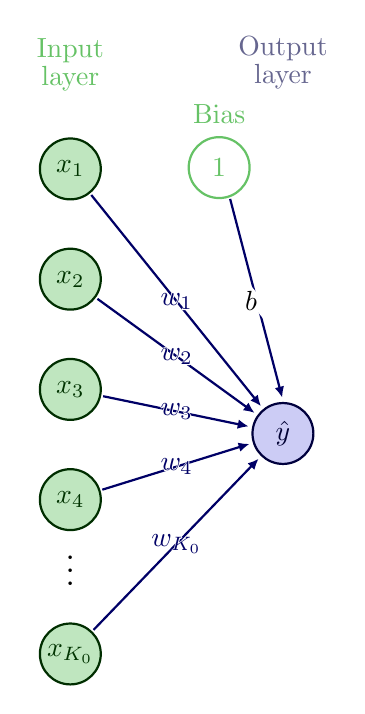
\begin{tikzpicture}[x=2.7cm,y=1.4cm]
  \message{^^JNeural network with arrows}
  \readlist\Nnod{4,5,5,5,3} % array of number of nodes per layer
  
  \def\NI{5} % number of nodes in input layers
  \def\NO{1} % number of nodes in output layers
  \def\yshift{0.4} % shift last node for dots
  
  % INPUT LAYER
  \foreach \i [evaluate={\c=int(\i==\NI); \y=\NI/2-\i-\c*\yshift; \index=(\i<\NI?int(\i):"K_0");}]
              in {1,...,\NI}{ % loop over nodes
    \node[node in,outer sep=0.6] (NI-\i) at (0,\y) {$x_{\index}$};
  }
  
  % BIAS TERM
  \node[node, above=200,align=center,mygreen!60!] at (1-0.3,1-4.8) {$1$};
  \draw[connect arrow] (\NO-0.25,\NO+0.24) -- (\NO,-0.6);
  \draw[connect,white,line width=4] (\NO-0.25,\NO-0.4) -- (\NO,0);
  \node[] at (1-0.15,0.3) {\contour{white}{$b$}};

  % OUTPUT LAYER
  \foreach \i [evaluate={\c=int(\i==1); \y=\NO/2-\i-\c*\yshift; \index=(\i<\NO?int(\i):"m");}]
    in {1}{ % loop over nodes
    \ifnum\i=1 % high-lighted node
      \node[node hidden]
        (NO-\i) at (1,\y) {$\hat{y}$};
      \foreach \j [evaluate={\index=(\j<\NI?int(\j):"K_0");}] in {1,...,\NI}{ % loop over nodes in previous layer
        \draw[connect ,white,line width=1.2] (NI-\j) -- (NO-\i);
        \draw[connect arrow] (NI-\j) -- (NO-\i)
          node[pos=0.50] {\contour{white}{$w_{\index}$}};
      }
    \fi
  }
  
  % DOTS
  \path (NI-\NI) --++ (0,1+\yshift) node[midway,scale=1.2] {$\vdots$};
  
% LABELS
  \node[above=200,align=center,mygreen!60!] at (NI-\NI) {Input\\[-0.2em]layer};
  \node[above=121,align=center,myblue!20!gray] at (NO-\NO) {Output\\[-0.2em]layer};
  \node[above=200,align=center,mygreen!60!] at (1-0.3,1-4.2) {Bias};

  
\end{tikzpicture}



\end{document}